\lecture{1}{09.03}
\section*{概述}%
\label{sec:概述}
\subsection*{资源}%
\label{sub:资源}
公众号:狗熊会、大数据文摘,好玩的数学

MOOC:爱课程,Coursera,Edx,网易公开课等

\subsection*{教师要求}%
\label{sub:教师要求}

教材:概率论与数理统计第二版

参考:The Lady Tasting Tea,程序员数学之概率统计,\ldots

学习目的:自问自答,自言自语

考核及成绩组成:\\期中(10)\\作业与考勤(10)\\期末(70)\\MOOC(10)

\subsection*{课程简介}%
\label{sub:课程简介}
概率:Probability

统计:Statistics

概率论与数理统计:Probability theory and Mathematical statistics

\begin{notation}
第一章重要但不突出
\end{notation}
从概率到概率论:新增时间(随机事件、样本空间变化)

从统计到数理统计:统计最开始为记录性质,后来衍生出预测,通过数学模型引入数理统计

类似的还有政府统计、经济统计等

2000-2015年间,IT时代逐渐转换为DT(Data Technology)时代,大数据逐渐占时代主体

{\centering{\section*{概率论部分}%
\label{sec:概率论部分}
}}
\section{第一章}%
\label{sec:第一章}

\subsection{随机事件}%
\label{sub:随机事件}
\subsubsection{现象}%
\label{subsub:现象}
确定性现象:一定条件下必然发生

随机现象强调统计规律性

\begin{notation}
统计规律性:

1. 每次试验前不能预测结果

2. 结果不止一个

3. 大量试验下有一定规律
\end{notation}
\begin{eg}
    星际旅行时宇航员看到的现象不是随机现象:

    对星际旅行的人而言,无法完成大量试验

    宇航员观测到的结果无规律,只能称为不确定现象(Uncertain)
\end{eg}
\begin{eg}
    扔一个骰子不能预测结果,但可以知道结果是$1,2,3,4,5,6$的一个,因此观察扔骰子是随机现象(Random)
\end{eg}
\subsubsection{随机试验}%
\label{subsub:随机试验}
随机试验(E):研究随机现象时进行的实验或观察等

\begin{notation}
    随机试验的特性:

    1. 可以在完全相同的条件下重复进行

    2. 试验的可能结果在试验前已知

    3. 试验的结果不可预测
\end{notation}
\subsubsection{样本}%
\label{subsub:样本}
在随机试验中,不可再分的最简单结果成为样本点$\omega$,全体样本点组成样本空间$\Omega$
\begin{notation}
    随机事件是基本事件的集合
\end{notation}
\begin{eg}
    扔骰子存在6个基本事件,可以产生$2^6$ 个随机事件,其中样本空间$\Omega=\{x|x\in \left[ 1,6 \right] ,x\in \mathbb{R}\}$
\end{eg}
\begin{eg}
    1. 射击时用$\omega_i$ 表示击中$i$ 环,样本空间为:\[
        \Omega=\{\omega_0,\omega_1,\omega_2,\ldots,\omega_{10}\}
    .\]

    2. 微信用户每天收到信息条数的取值范围是$\left[ 0,+\infty \right) $,样本空间为无限集:\[
        \Omega=\left\{ N|N\ge 0 ,N\in \mathbb{R}\right\} 
    .\] 

    3. 电视机的寿命样本空间为$\Omega=\left\{ t|t>0 \right\} $,为连续的非负实数集

    4. 投掷两枚硬币,样本空间为$\Omega=\left\{ \left( x,y \right) |x,y=0,1 \right\} $,其中$0,1$ 分别代表正面和背面
\end{eg}
\begin{notation}
    1. 样本点可以不是数

    2. 样本空间可以是无限集
\end{notation}
\subsubsection{随机事件}%
\label{subsub:随机事件}
\subsection{事件关系与运算}%
\label{sub:事件关系与运算}
1.1. $A\subset B$:$A$ 发生必然$B$ 发生

1.2. $A=B$ :$A\subset B, B\subset A$ 

2. $A\cup B$:$A$ 和$B$ 至少有一个发生

2.1 $A_1\cup A_2\cup \ldots\cup A_n=\bigcup_{i=1}^{n}A_1$

3. $A\cap B$:$A$ 和$B$ 只发生一个

4.1. $A,B$互斥:不能同时发生: $AB=\varnothing$

4.2. $A,B$对立:非此即彼:$A\cup B=\Omega$

5. $A-B$:$A \bar{B}$或$A(\Omega-B)$,或$A$ 发生但$B$ 不发生
\begin{notation}
    $A-B=A\bar{B}\subset A$,$B-A=B\bar{A}\subset B$

    当$AB=\varnothing$ 时,$A-B= A,B-A=B$
\end{notation}

\begin{notation}
    $P\left( \Omega \right) =1,P\left( \varnothing \right) =0$,且$P\left( \Omega \right) +P\left( \varnothing \right) =1$ ,即$\Omega$ 与$\varnothing$ 互斥
\end{notation}

6. 结合律:$\left( A\cup B \right) \cup C = A\cup \left( B\cup C \right) $

7. 分配律:$\left( AB \right) \cup C=\left( A\cup C \right) \left( B\cup C \right) $ ,$\left( AUB \right) C =AC\cup BC$

8. 交换律:$A\cup B=B\cup A,AB=BA$
\begin{notation}
    德摩根律:\[
    \overline{\bigcup_{i=1}^{n}A_i} = \bigcap_{i=1}^{n}\overline{A_i}
    .\] 
    \[
        \overline{\bigcap_{i=1}^{n}A_i}=\bigcup_{i=1}^{n}\overline{A_i}
    .\] 
\end{notation}
\begin{eg}
     \[
        \overline{A\cup B}=\bar{A}\bar{B}
    .\]
    \[
        \overline{\left( A\cup B \right) \cup C} = \overline{A\cup B}\bar{C}=\ldots
    .\] 
    \[
        \overline{A\cap B}=\bar{A}\cup \bar{B}
    .\] 
\end{eg}
\subsection{事件的概率}%
\label{sub:事件的概率}
概率分类:
\begin{align*}
    \begin{cases}
        \text{主观概率}\\ 
        \text{统计概率}\\
        \text{古典概型}\\
        \text{几何概型}
    \end{cases}
.\end{align*}
\begin{notation}
    德摩根、蒲丰、皮尔逊、维纳均进行过投掷硬币的试验,随着试验次数的增加,出现正面的频率逐渐接近0.5

    大数定律说明,该事件的概率为0.5
\end{notation}
\begin{defi}
    统计概率:$A$为试验$E$的一个事件,随着重复次数$n$的增加,$A$的频率接近于某个常数$p$,定义事件$A$的概率为$p$,记为$P\left( A \right) =p$
\end{defi}
频率的特性:

1. 非负性:$f_n\left( A \right) \in \left[ 0,1 \right] $

2. 规范性:$f_n\left( \Omega \right) =1$

3. 有限可加性:$A_i$ 两两互斥,则$f_n\left( \sum_{i=1}^{n} A_i \right) =\sum_{i=1}^{n} f_n\left( A_i \right) $
\begin{defi}
    主观概率:人对某个事件发生与否的可能性的估计
\end{defi}

\begin{defi}
    完备事件组:$A_1,A_2,\ldots,A_n$两两互斥,且\[
        P\left( \sum_{i=1}^{n} A_i \right) =1
    .\] 或\[
        \sum_{i=1}^{n} A_i=\Omega
    .\] 则称$A_1\to A_n$ 为完备事件组(不重不漏)
\end{defi}
\begin{eg}
    $A,\bar{A}$ 是完备事件组
\end{eg}
\subsubsection{古典概型}%
\label{subsub:古典概型}
古典概型特点:有限等可能性(基本事件数有限,基本事件发生的可能性相等)
\begin{notation}
    概率计算:\[
        P\left( A \right) =\frac{m}{n} = \frac{n\left( A \right) }{n\left( \Omega \right) }
    .\] 
\end{notation}
\begin{eg}
    某年级有6人在9月份出生,求6个人中没有人同一天过生日的概率

    基本事件总数:$30^6$

    目标事件: $30\cdot 29\cdot 28\cdot 27\cdot 26\cdot 25=P_{30}^{6}$ 

    概率:\[
        P\left( A \right) =\frac{\mathrm{P}_{30}^{6}}{30^6}
    .\] 
\end{eg}
\begin{eg}
    有$N$个乒乓球中有$M$个白球、$N-M$个白球,任取$n(n<N)$个球,分有放回和不放回,求取到$m$个黄球的概率

    1. 不放回:

    基本事件总数: $\mathrm{C}_{N}^{n}$ 

    目标事件:$\mathrm{C}_{M}^{m}\mathrm{C}_{N-M}^{n-m}$ 

    概率: \[
        P=\frac{\mathrm{C}_{M}^{m}\mathrm{C}_{N-M}^{n-m}}{\mathrm{C}_{N}^{n}},n=\max\left\{ 0,n-\left( N-M \right)  \right\}, \ldots,\min\left\{ n,M \right\} 
    .\] 

    2. 有放回:

    \[
    P=\frac{\mathrm{C}_{n}^{m}M^m\left( N-M \right) ^{n-m}}{N^n}=\mathrm{C}_{n}^{m}\left( \frac{M}{N} \right) ^m\left( 1-\frac{M}{N} \right) ^{n-m},m\in \left[ 0,n \right]
    .\] 
    注意到该概率为伯努利分布$\mathrm{C}_{n}^{m}B\left( n,\frac{M}{N} \right) $
\end{eg}
匹配问题:
\begin{eg}
    麦克斯韦-玻尔兹曼统计问题:

    $n$个质点随机落入$N\left( N>n \right) $ 个盒子,盒子容量不限,设$A$ 表示指定的$n$个盒子各有一个质点,$B$ 表示恰好有$n$个盒子装一个质点

    基本事件总数:$N^n$ 

    $A$考虑顺序,即:\[
        P\left( A \right) =\frac{n!}{N^n}
    .\] 

    同理:\[
        P\left( B \right) =\frac{\mathrm{C}_{N}^{n}}{N^n}
    .\] 
\end{eg}        
\subsubsection{几何概型}%
\label{subsub:几何概型}
几何概型特点:使用事件所对应的\textbf{几何度量}计算
\[
    P\left( A \right) =\frac{m\left( A \right) }{m\left( \Omega \right) }
.\] 
\begin{notation}
    度量:面积、体积、长度等描述几何量大小的测度方式
\end{notation}
\begin{eg}
    地面铺满2 dm的地砖,向地面投掷一个$r=0.5$ dm的光盘,求光盘不与边线相交的概率
\end{eg}
如图:
\begin{center}
    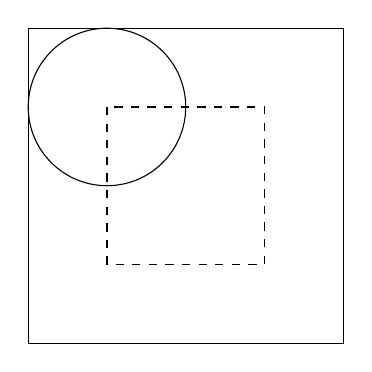
\begin{tikzpicture}
        \draw [] (-2,2) rectangle (2,-2);
        \draw [] (-1,1) circle [radius=1] node at(-1,1) {};
        \draw [dashed] (-1,1) rectangle (1,-1);
    \end{tikzpicture}
\end{center}
课后习题:A组8题,B组3题
\begin{eg}
    两人相约8-9点间在某地相见,先到的人等待20分钟后离去,求二人会面的概率

    设$\left( x,y \right) $ 分别表示两人到达的时刻

    设G为样本空间,绘制样本空间:
    \begin{center}
        \begin{tikzpicture}[xscale=0.5,yscale=0.5]
            % Axis
            \node [anchor=north east] (O) at(0,0) {$O$};
            \draw [->] (0,0)--(0,7)  node [above] {$y$};
            \draw [->] (0,0)--(7,0) node [right] {$x$};

            \draw [] (0,0) rectangle (6,6) node at(5,5) {$G$};
        \end{tikzpicture}
    \end{center}

    由题:两人到达的时间之差的绝对值小于20分钟($\frac{1}{3}$ 小时),即:\[
        |x-y|\le \frac{1}{3}
    .\] 
    将事件绘制:
    \begin{center}
        \begin{tikzpicture}[xscale=0.5,yscale=0.5]
            % Axis
            \draw [->] (0,0)--(0,7)  node [above] {$y$};
            \draw [->] (0,0)--(7,0) node [right] {$x$};
            \node [anchor=north east] (O) at(0,0) {$O$};

            \draw [] (0,0) rectangle (6,6) node at(5,1) {$G$};
            \draw [dashed] (2,0)--(6,4);
            \draw [dashed] (0,2)--(4,6);
            \node [] (g) at (3,3) {$g$};
        \end{tikzpicture}
    \end{center}
    \[
        P\left( g \right) =\frac{m\left( g \right) }{m\left( G \right) }=\frac{S\left( g \right) }{S\left( G \right) }=\frac{1-\left( \frac{2}{3} \right) ^2}{1}=\frac{4}{9}
    .\] 
\end{eg}
\begin{notation}
    几何概型的特点:

    1. 非负性:\[
        P\left( A \right) \in \left[ 0,1 \right] 
    .\] 

    2. 规范性:\[
        P\left( \Omega \right) =1
    .\] 

    3. 可列可加性: \[
        P\left( \sum_{i=1}^{n} A_i \right) =\sum_{i=1}^{n} P\left( A_i \right) 
    .\] 
\end{notation}
